% =====================================================================
%  IRC 2026 (SLTC) camera-ready full paper
%  A Gamified Upper Limb Stroke Rehabilitation System with Remote
%  Monitoring and Communication Features
%
%  Layout follows "Camera_ready_template_IRC_SLTC_2026": A4, print area
%  17.3 cm x 24.3 cm, two 8.25 cm columns 0.8 cm apart, Times 10 pt,
%  no page numbers, IEEE numbered references, 6-8 pages.
%
%  Compile with pdfLaTeX or XeLaTeX (Overleaf: upload this folder, main
%  file report.tex). Diagrams 1, 3, 4 and 5 are Mermaid sources in
%  diagrams/*.mmd, rendered to figures/*.pdf by diagrams/build.sh.
% =====================================================================
\documentclass[10pt,a4paper,twocolumn]{article}

% ---- Page layout: margins 2.54 / 2.86 cm top / bottom, 1.85 cm sides --
\usepackage[a4paper,top=25.4mm,bottom=28.6mm,left=18.5mm,right=18.5mm,
            columnsep=8mm,headheight=0pt,headsep=0pt,footskip=0pt]{geometry}
\usepackage[T1]{fontenc}
\usepackage[utf8]{inputenc}
\usepackage{amsmath}
\usepackage{newtxtext,newtxmath}          % Times New Roman
\usepackage{graphicx}
\usepackage{array,tabularx}
\usepackage{enumitem}
\usepackage{titlesec}
\usepackage{caption}
\usepackage{eso-pic}
\usepackage{xcolor}
\usepackage{url}                          % URLs typeset, never active links
\usepackage{cite}                         % [1], [2] sorted; ranges as [1]-[3]
\usepackage{flafter}                      % no float before its first citation
\usepackage{flushend}                     % balance the columns on the last page

\pagestyle{empty}                         % no page numbers
\setlength{\parindent}{12pt}              % 1 pica
\setlength{\parskip}{0pt}
\emergencystretch=1em
\raggedbottom
\usepackage{indentfirst}

% ---- Conference logo, top right of every page ------------------------
\AddToShipoutPictureBG{%
  \AtPageUpperLeft{%
    \put(\LenToUnit{\paperwidth-18.5mm-40mm},\LenToUnit{-21mm}){%
      
\includegraphics[width=40mm]{figures/irc2026_logo.png}}}}

% ---- Headings -----------------------------------------------------------
% First level: I., II., ... small caps, centred, 12 pt before, 6 pt after.
% Second level: A., B., ... italic, flush left, 9 pt before, 3 pt after.
\setcounter{secnumdepth}{2}
\renewcommand{\thesection}{\Roman{section}}
\renewcommand{\thesubsection}{\thesection-\Alph{subsection}}   % cited as "Section III-B"
\titleformat{\section}{\normalfont\normalsize\scshape\centering}{\thesection.}{0.5em}{}
\titlespacing*{\section}{0pt}{12pt}{6pt}
\titleformat{\subsection}{\normalfont\normalsize\itshape}{\Alph{subsection}.}{0.5em}{}
\titlespacing*{\subsection}{0pt}{9pt}{3pt}

% ---- Captions (template "Caption" style: 9 pt bold) --------------------
\DeclareCaptionLabelSeparator{dotsp}{.\ }
\captionsetup{font={small,bf},labelsep=dotsp}
\captionsetup[figure]{name=Fig.,justification=justified,singlelinecheck=false,skip=6pt}
\captionsetup[table]{name=Table,justification=centering,skip=6pt,position=top}
\setlength{\textfloatsep}{10pt plus 2pt minus 2pt}
\setlength{\floatsep}{8pt plus 2pt minus 2pt}

% ---- Lists: rounded bullets; numbered list for ordered items -----------
\setlist[itemize]{label=\textbullet,leftmargin=18pt,itemsep=0pt,topsep=2pt,parsep=0pt}
\setlist[enumerate]{label=\arabic*.,leftmargin=18pt,itemsep=0pt,topsep=2pt,parsep=0pt}

% ---- Tables: 9 pt text, 9 pt bold heads ---------------------------------
\newcolumntype{Y}{>{\raggedright\arraybackslash}X}
\newcolumntype{L}[1]{>{\raggedright\arraybackslash}p{#1}}
\newcolumntype{C}[1]{>{\centering\arraybackslash}p{#1}}
\newcommand{\tablefont}{\small\renewcommand{\arraystretch}{1.1}\setlength{\tabcolsep}{3pt}}
\newcommand{\hd}[1]{\textbf{#1}}

\begin{document}

% =====================================================================
\twocolumn[{%
\begin{center}
{\fontsize{24}{28}\selectfont A Gamified Upper Limb Stroke Rehabilitation System with Remote Monitoring and Communication Features\par}
\vspace{12pt}
{\fontsize{11}{13}\selectfont M. Imzan\textsuperscript{1*}, M. Atheeq\textsuperscript{1}, D. Karunakalage\textsuperscript{2}, V. Herath\textsuperscript{1}\par}
\vspace{6pt}
{\itshape
\textsuperscript{1}Department of Electronics \& Telecommunication, Faculty of Engineering, Sri Lanka Technology Campus, Padukka 10500, Sri Lanka\par
\vspace{3pt}
\textsuperscript{2}Department of Electrical Engineering, Faculty of Engineering, Sri Lanka Technology Campus, Padukka 10500, Sri Lanka\par}
\vspace{3pt}
\textsuperscript{1}22ug2-0072@sltc.ac.lk*, \textsuperscript{1}22ug2-0237@sltc.ac.lk, \textsuperscript{2}dulashik@sltc.ac.lk, \textsuperscript{1}vihanga.h@sltc.ac.lk\par
\vspace{14pt}
\end{center}
}]

\noindent\textbf{\textit{Abstract - Stroke often leaves lasting weakness in the arm and hand, and recovery depends on frequent, repetitive practice that patients find hard to sustain at home. This paper presents a low cost, gamified upper limb rehabilitation system that combines webcam based hand tracking with a single channel forearm electromyography sensor connected to an ESP32 microcontroller. MediaPipe hand landmarks give seven hand and wrist movements that control four games with rewards and adaptive difficulty, while the electromyography signal is attached to every game command as a measure of muscle activity. Every session is stored locally and reviewed by the physiotherapist in a web application. Offline movement classification from electromyography was tested on nine healthy volunteers, each unseen during training. Over seven movements, against a chance level of 14.3\%, a support vector machine on 200 millisecond windows reached 37.2\% accuracy, longer 5.12 second windows raised this to 47.3\%, and features from the frozen MOMENT-1 time-series foundation model with a random forest gave the best accuracy of 48.1\%. Rest, hand opening and hand closing were recognized far better than the wrist directions, which supports letting the camera decide each movement while electromyography provides activity feedback.}}

\vspace{10pt}
\noindent\textbf{\textit{Keywords - Electromyography, hand tracking, serious games, time-series foundation models}}

% =====================================================================
\section{Introduction}

Stroke is one of the most common causes of long term disability in adults worldwide~\cite{gbd2024}. Most survivors are left with lasting problems in arm and hand movement, which make activities of daily living such as eating, dressing and washing harder. Good recovery needs frequent, repeated and task specific practice, which is hard to keep up with regular therapy alone~\cite{winstein2018}, and sensor and game based rehabilitation can make therapy more engaging, accessible and measurable~\cite{doumas2021}. Electromyography (EMG) sensors detect muscle activity even when visible movement is very small~\cite{munoz2022}, and webcam based hand tracking shows the position of the hand and fingers without any wearable device~\cite{zhang2020}.

Current practice has several problems. Repeating the same exercises bores patients, so adherence falls once supervision stops~\cite{winstein2018}. Patients far from cities often cannot reach trained therapists~\cite{lee2018}. Many technical solutions do only one thing, for example tracking hand gestures, without combining game based engagement with clinician monitoring~\cite{zondervan2016,song2019}, and regular therapy rarely produces numeric progress data that a clinician can follow between visits. Tele rehabilitation platforms exist~\cite{lee2018,marin2021}, but few combine a real time game interface, muscle activity sensing and clinical monitoring in one low cost system.

The aim of this work is a low cost rehabilitation game platform that recognizes therapeutic hand and wrist movements from webcam and EMG data, uses them to control interactive games, and lets physiotherapists monitor patients. The objectives are as follows:
\begin{enumerate}
\item To develop hardware for the synchronous capture of hand movement and muscle activity.
\item To design feature extraction and classification methods that identify hand movements from the sensor data.
\item To develop interactive rehabilitation games and measure the accuracy of patient movements.
\item To develop a web platform that lets physiotherapists monitor progress and communicate with patients.
\end{enumerate}

Table~\ref{tab:status} separates the completed parts from future work. Section~II reviews related work, Section~III describes the system and experiments, Section~IV presents and discusses the results, and Section~V concludes the paper.

\begin{table}[!t]
\caption{Status of the work}\label{tab:status}
\tablefont
\begin{tabularx}{\columnwidth}{|L{15mm}|Y|}
\hline
\hd{Status} & \hd{Components}\\\hline
Completed & Battery powered EMG hardware and ESP32 firmware with a USB serial link; webcam detection of seven movements; fusion of camera labels with EMG features; four games with rewards and adaptive difficulty; local server, database and offline queue; physiotherapist web application; EMG dataset from nine healthy volunteers; offline comparison of classical and foundation model classifiers; 47 automated tests\\\hline
Future work & Enclosure and Wi-Fi transmission; patient login, patient--physiotherapist text and voice messaging, and remote access; EMG activity levels in game control; measurement of webcam accuracy, latency and usability; stroke patient data after ethics approval\\\hline
\end{tabularx}
\end{table}

% =====================================================================
\section{Literature Review}

\subsection{Wearable Sensing and Serious Games}

Inertial measurement units (IMUs) describe large arm movements well~\cite{yin2018,lee2018}, while surface EMG records muscle activity that can reveal movement intention even when voluntary movement is very limited~\cite{jiang2018}. A meta analysis found that EMG based interventions can improve upper limb function after stroke, although evidence of superiority over equal amounts of conventional therapy is limited~\cite{munoz2022}. Low cost EMG has been used at home: Tele-REINVENT rewarded wrist extension in games guided by a therapist over video calls~\cite{marin2021,marin2022}, and MyoGuide evaluated mobile EMG guided wrist training in subacute stroke~\cite{lin2024}. Combining IMUs with EMG improves gesture recognition~\cite{jiang2018} but adds cost and calibration. Serious games improved upper limb function more than conventional therapy in a meta analysis of randomized trials~\cite{doumas2021}; robotic games have combined motor and cognitive training~\cite{heins2017}; and good games follow motor learning principles of task specific repetition, feedback and gradually increasing difficulty~\cite{song2022}. Ibrahim et al.\ combined Kinect tracking, games and EMG monitoring, but tested only healthy participants~\cite{ibrahim2024}.

\subsection{Hand Tracking and Movement Recognition}

MediaPipe Hands detects 21 hand landmarks in real time from a single RGB camera~\cite{zhang2020}, and has been used for remote hand rehabilitation with deep learning feedback~\cite{dhuzuki2025}. A camera cannot, however, measure how strongly a muscle is activated. For EMG, time domain features such as mean absolute value and waveform length with Linear Discriminant Analysis (LDA) or Support Vector Machines (SVM) are standard for real time control~\cite{geng2017}, random forests are robust to features on different scales~\cite{breiman2001}, and deep networks need more data and computing power~\cite{panwar2019}. Classifiers often fail when the electrode position, arm position or user changes~\cite{geng2017}.

\subsection{Time-Series Foundation Models}

MOMENT is a family of open transformer models pre-trained on a large collection of public time series, which classifies fixed length inputs of 512 steps~\cite{goswami2024}. It can be used frozen, with a classifier on its embeddings, or fine-tuned with low-rank adaptation (LoRA), which trains small matrices added to the attention layers~\cite{hu2022}. MOMENT normalizes each window with reversible instance normalization (RevIN)~\cite{kim2022}, which removes its mean and scale; for an EMG envelope, where activity level separates movements, this may remove useful information. Public EMG datasets such as UCI EMG Data for Gestures~\cite{lobov2018} could add training data but use different sensors.

\subsection{Tele Rehabilitation and Research Gap}

Tele rehabilitation systems combine a sensor, a data link and a remote monitoring platform~\cite{lee2018,marin2021}, but few combine games, muscle sensing and two way communication with the therapist (Table~\ref{tab:related}). Multi sensor systems~\cite{yin2018,jiang2018} cost more and are harder to set up at home, while many game systems~\cite{heins2017,ibrahim2024} offer no clinical monitoring. There is also little evidence on how much movement information one low cost EMG envelope channel carries, or whether foundation models help with such small datasets. This work addresses both points.

\begin{table}[!t]
\caption{Comparison of related rehabilitation systems}\label{tab:related}
\tablefont
\begin{tabularx}{\columnwidth}{|L{25mm}|Y|C{8mm}|L{16.5mm}|}
\hline
\hd{Study} & \hd{Sensing} & \hd{Game} & \hd{Monitoring}\\\hline
Yin \& Xu~\cite{yin2018} & IMU & Yes & No\\\hline
Jiang et al.~\cite{jiang2018} & EMG + IMU & No & No\\\hline
Heins et al.~\cite{heins2017} & Robotic device & Yes & Not reported\\\hline
Lee et al.~\cite{lee2018} & Wearable IMU & No & Yes\\\hline
Marin-Pardo et al.~\cite{marin2021} & EMG & Yes & Video calls\\\hline
Ibrahim et al.~\cite{ibrahim2024} & Kinect + EMG & Yes & No\\\hline
Dhuzuki et al.~\cite{dhuzuki2025} & Camera & No & Yes\\\hline
Proposed & Webcam + EMG & Yes & Clinic\newline dashboard\\\hline
\end{tabularx}
\end{table}

% =====================================================================
\section{Methodology}

\subsection{System Architecture}\label{ss:arch}

The system has four layers (Fig.~\ref{fig:arch}): sensing (the EMG sensor with an ESP32, and a webcam), processing (EMG and vision pipelines and a fusion engine), application (four games) and data and monitoring (a local application programming interface (API), a database and the web application). Everything runs on one laptop. The game process runs three threads: an EMG thread that reads the serial port, a vision thread that processes every camera frame, and a fusion thread that every 50~ms combines the latest camera label and EMG features into one command for the game loop, which runs at 30 frames per second. A FastAPI server with an SQLite database stores patients, sessions and attempts and serves the web application, which starts and stops the games. A session that ends while the server is down is kept in an offline queue and uploaded later.

\begin{figure}[!t]
\centering
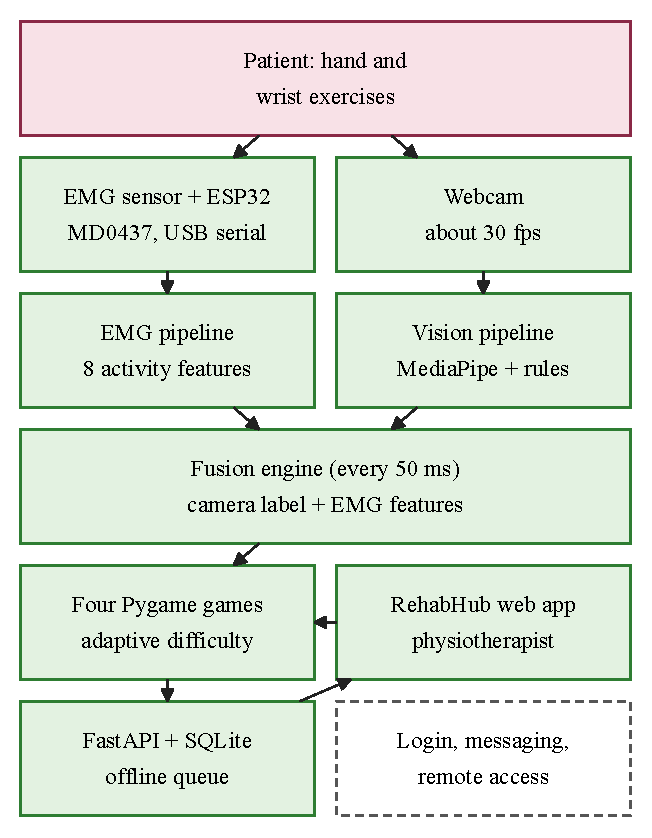
\includegraphics[width=0.92\columnwidth]{figures/fig1_architecture.pdf}
\caption{System architecture (green: completed; dashed: future work)}\label{fig:arch}
\end{figure}

\subsection{Hardware}\label{ss:hw}

Fig.~\ref{fig:hw} shows the acquisition hardware. The MD0437 single channel surface EMG module amplifies, rectifies and smooths the muscle signal on board, so its output is an activity envelope rather than raw EMG. It is powered from a split $\pm$9~V battery supply and never connected to mains while worn. Three disposable Ag/AgCl electrodes are used: signal $+$ on the upper forearm muscle, signal $-$ 3--4~cm towards the wrist, and the reference on the bony area near the elbow. The module output is read on GPIO34 (ADC1) of a 30-pin ESP32 with 12-bit resolution (0--4095) and 11~dB attenuation, and each sample is sent to the laptop as the line ``timestamp (ms), ADC value'' over USB serial at 921600~baud. The dataset in Section~\ref{ss:data} was recorded at 100~Hz; the current firmware samples at 1~kHz with a microsecond timer. Lines that are malformed or outside 0--4095 are discarded, and games that use EMG pause if no valid sample arrives for 2.5~s.

\begin{figure}[!t]
\centering
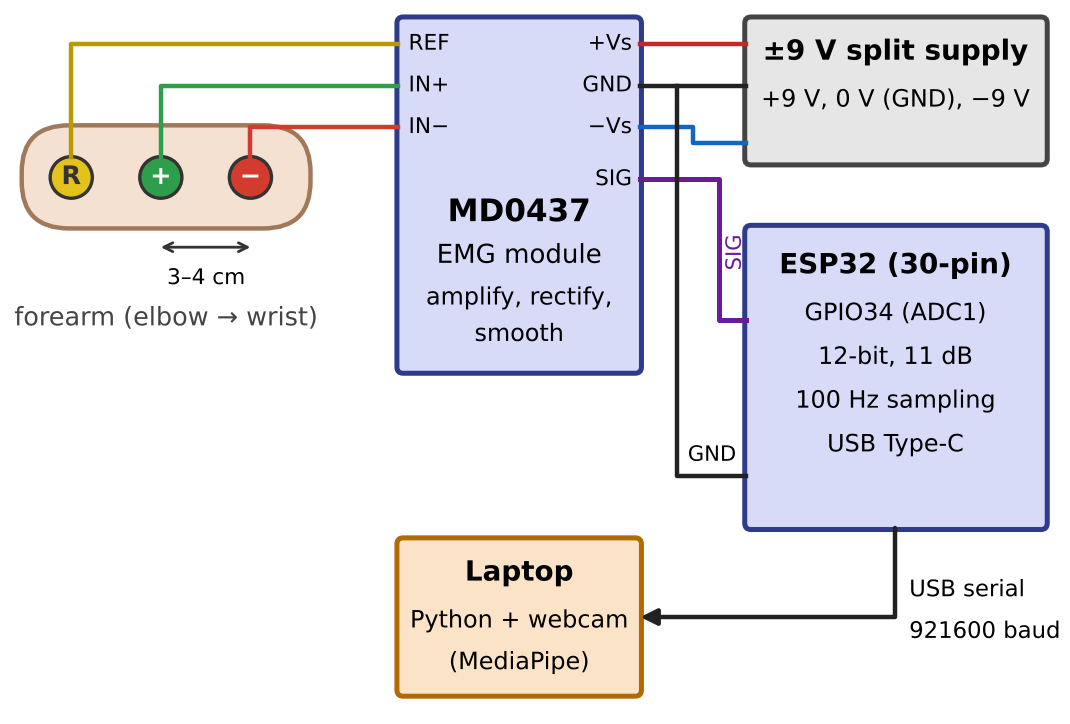
\includegraphics[width=\columnwidth]{figures/fig2_hardware.png}
\caption{Wiring of the EMG acquisition hardware, as used to record the dataset at 100 Hz}\label{fig:hw}
\end{figure}

\subsection{Visual Hand Detection}\label{ss:vision}

Each webcam frame is processed with the MediaPipe hand landmarker~\cite{zhang2020}, which returns 21 landmarks. From these, the system computes the curl angle of each finger, the fingertip reach divided by the palm size (so that the rules work at any camera distance), the thumb to index pinch ratio, and a strict full fist flag. A pinch ratio below 0.34 or one or no extended finger gives Hand Close, three or more extended fingers give Hand Open, and anything else gives Rest. A label is kept only when 3 of the last 5 frames agree. Left, Right, Up and Down come from movement of the palm center relative to an anchor point, beyond 2.5\% of the frame width or 4\% of its height; a direction is held for 350~ms, and closing the hand resets the anchor. A smoothed pointer at the middle finger is used for aiming and steering.

\subsection{EMG Processing and Features}\label{ss:emg}

Because the MD0437 output is an envelope, the 20--450~Hz band pass and 50~Hz notch filters needed for raw EMG are skipped. The signal is cut into 200~ms windows every 100~ms ($N=20$ samples at 100~Hz, 200 at 1~kHz), and eight features are computed per window: root mean square (RMS), mean absolute value (MAV), variance, standard deviation, peak, waveform length (WL), zero crossings and slope sign changes. The three main features are
\begin{equation}\label{eq:mav}
\mathit{MAV} = \frac{1}{N}\sum_{i=1}^{N} |x_i|,
\end{equation}
\begin{equation}\label{eq:rms}
\mathit{RMS} = \sqrt{\frac{1}{N}\sum_{i=1}^{N} x_i^{2}},
\end{equation}
\begin{equation}\label{eq:wl}
\mathit{WL} = \sum_{i=2}^{N} |x_i - x_{i-1}|,
\end{equation}
where $x_i$ is the $i$-th envelope sample (ADC value) in a window of $N$ samples. These values describe electrical activity in ADC units; they rise with contraction but are not calibrated muscle force. The same code serves the live system and the offline experiments (Fig.~\ref{fig:pipe}).

\begin{figure}[!t]
\centering
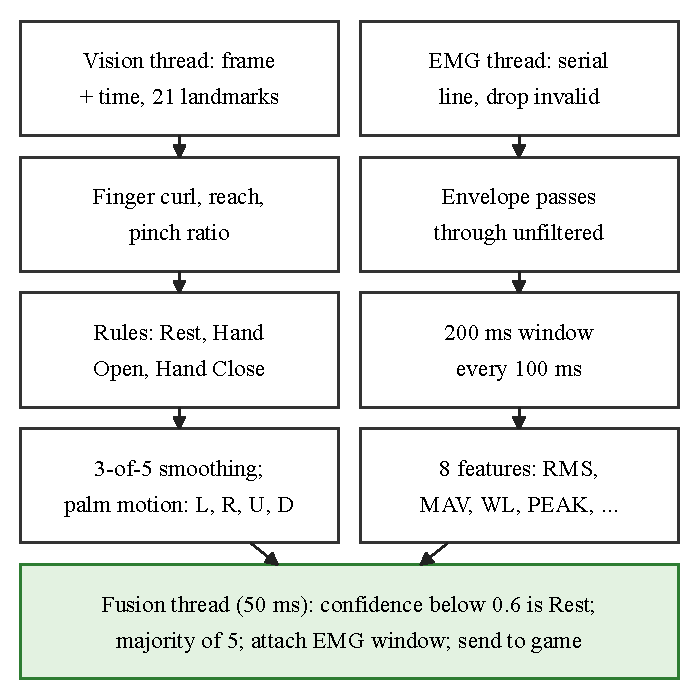
\includegraphics[width=0.92\columnwidth]{figures/fig3_pipeline.pdf}
\caption{Vision, EMG and fusion pipelines; each runs in its own thread}\label{fig:pipe}
\end{figure}

\subsection{Fusion of Camera and EMG}\label{ss:fusion}

Every 50~ms the fusion thread takes the latest camera label, replaces it with Rest when its confidence is below 0.6, takes a majority vote over the last five labels, and attaches the latest EMG window and the camera frame's capture time. The earlier design fired a game action only when both signals agreed. This was changed because a single forearm channel separates activity levels well but carries little information about direction (Section~\ref{ss:res-class}). EMG therefore never overrides a camera label; it is shown as live activity feedback, stored with every attempt, and in Webcam + EMG mode the games wait for fresh EMG data. The stored capture time allows the camera to game delay to be measured for every command.

\subsection{Dataset}\label{ss:data}

Nine healthy adult volunteers (S01--S09), who took part voluntarily and gave informed consent, performed each of the seven movements for about 60~s with the forearm resting on a table, recorded at 100~Hz. The dataset has 61 files and 369,435 labelled samples; files containing several recordings or gaps over 1~s were split into 66 segments so that no window spans two recordings. Two volunteers each miss one movement (S01 Rest, S04 Down), and S01 lost 26--50\% of its samples to a lossy recording link. The 200~ms windows give 36,873 examples.

\subsection{EMG Movement Classification}\label{ss:models}

The classifiers were studied offline to decide what role EMG should play; none of them controls the games. Each assigns a window to one of the seven movements (Fig.~\ref{fig:models}). First, LDA, SVM with a radial basis function kernel ($C=10$), and a random forest with 200 trees were trained on the eight features of the 200~ms windows.

Second, because MOMENT-1 needs 512 evenly spaced samples, each segment was resampled to a 10~ms grid with dropped samples filled by linear interpolation, S01 was excluded (39\% interpolated), and every sample $x$ of subject $s$ was transformed and calibrated as
\begin{equation}\label{eq:calib}
z = \operatorname{clip}\!\left(\frac{\ln(1+x) - \mu_s}{\sigma_s},\,-6,\,6\right),
\end{equation}
where $\mu_s$ and $\sigma_s$ are the mean and standard deviation of $\ln(1+x)$ over all of that subject's recordings, computed without labels. The logarithm keeps the quiet Rest and the strong Hand Close on one scale, and the calibration removes gain differences between people. Windows of 512 samples (5.12~s) were cut every 128 samples, giving 2,494 windows from eight volunteers, and the same eight features were also computed on them.

Third, MOMENT-1-small (35.3 million parameters)~\cite{goswami2024} was used frozen, with its untrained head or with LDA, SVM or random forest on its 512 value embedding, using \eqref{eq:calib} in place of RevIN~\cite{kim2022} or, for comparison, RevIN itself. Fourth, it was fine-tuned as a linear probe (only the 3,591 parameter head trained) and with rank 8 LoRA~\cite{hu2022} adapters on the attention query and value projections (118,279 parameters), each for up to 15 epochs with early stopping. Finally, the UCI dataset~\cite{lobov2018} (36 people, eight channel armband) was converted to envelope-like windows and used either as extra training windows for the three shared movements or to pre-train the LoRA adapters.

Data were always split by subject, because overlapping windows are near duplicates. The main test is leave-one-subject-out (LOSO) over S02--S09: each fold tests one volunteer, trains on six and uses the last for early stopping. A holdout split (train S02--S05, validate S06, test S07--S09) gives a second view. Accuracy and the macro F1-score are reported, with chance at $1/7 = 14.3\%$:
\begin{equation}\label{eq:f1}
\mathrm{F1}_{\mathrm{macro}} = \frac{1}{K}\sum_{k=1}^{K}\frac{2P_kR_k}{P_k+R_k},
\end{equation}
where $P_k$ and $R_k$ are the precision and recall of class $k$ and $K=7$.

\begin{figure*}[!t]
\centering
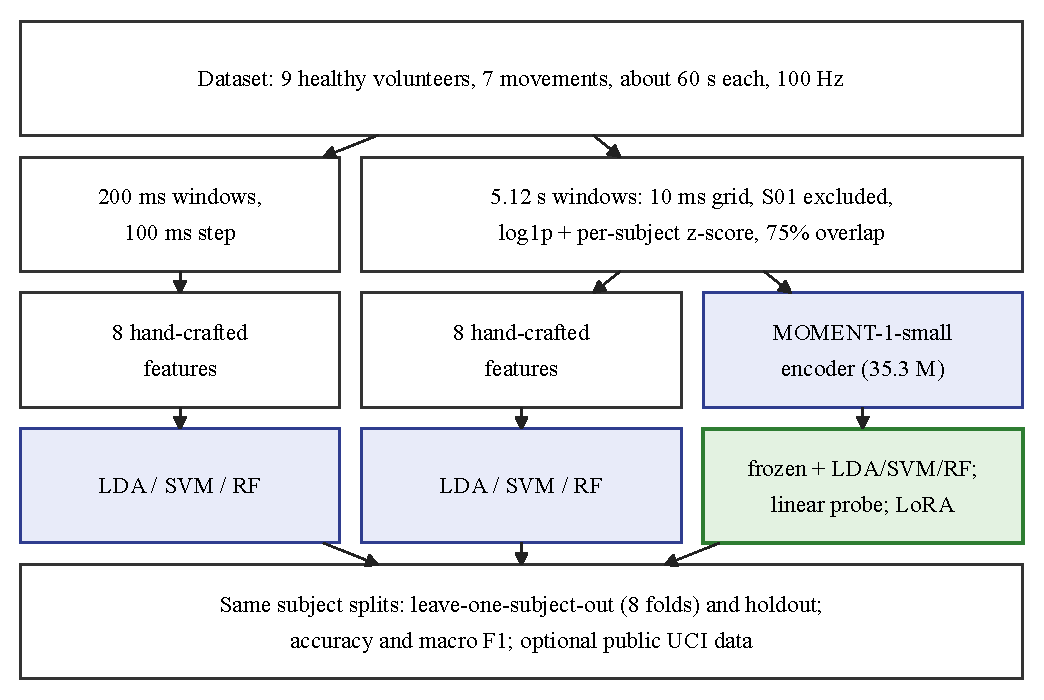
\includegraphics[width=0.62\textwidth]{figures/fig4_models.pdf}
\caption{Offline EMG classification pipelines compared on the same subject splits (green: classifiers built on MOMENT-1; frozen MOMENT-1 features with a random forest gave the best result)}\label{fig:models}
\end{figure*}

\subsection{Games and Adaptive Difficulty}\label{ss:games}

Four games were written in Python with Pygame and are launched from the web application (Table~\ref{tab:games}). Following motor learning principles~\cite{song2022}, movements map naturally to game actions, sound and visual feedback is immediate, and difficulty increases gradually. Each game asks for one target movement at a time and records the target, the detected movement, correctness, reaction time, EMG RMS and MAV, and confidence. Every game can also be played with the keyboard or a simulator.

\begin{table}[!t]
\caption{Games and webcam controls}\label{tab:games}
\tablefont
\begin{tabularx}{\columnwidth}{|L{12mm}|Y|L{19mm}|}
\hline
\hd{Game} & \hd{Webcam control} & \hd{Trains}\\\hline
Balloon Pop & Aim with the hand; a full fist on the balloon pops it & Reaching, hand close and open\\\hline
Car Driving & Hand left, middle or right picks one of three lanes; a fist brakes & Side to side reach, hand close\\\hline
Treasure Hunt & Push the hand like a joystick to walk; open, then close at each chest & Four directions, hand open and close\\\hline
Shape Matching & Fist to grasp a shape, carry it, open to drop it in its hole & Grasp, release, precise reach\\\hline
\end{tabularx}
\end{table}

A correct movement scores 10 points, plus 5 while three or more are correct in a row, with game specific bonuses. A session lasts 180~s by default and ends with a results screen showing score, accuracy, best streak, reaction time and one to three stars. Movement accuracy is
\begin{equation}\label{eq:ma}
\mathit{MA} = \frac{S}{T}\times 100\%,
\end{equation}
where $S$ is the number of correct attempts and $T$ the total number of attempts. Because the EMG envelope is not a calibrated force and relates weakly to movement, difficulty adapts to accuracy instead of an EMG calibration, which also works in every input mode. Levels run continuously from 1.0 to 5.0. In automatic mode (Fig.~\ref{fig:session}), after at least four attempts since the last change, the level $\ell$ is updated from the accuracy $a_6$ of the last six attempts:
\begin{equation}\label{eq:level}
\ell \leftarrow
\begin{cases}
\min(\ell + 0.5,\ 5), & a_6 \ge 80\%,\\
\max(\ell - 0.5,\ 1), & a_6 \le 40\%,\\
\ell, & \text{otherwise}.
\end{cases}
\end{equation}
Each game interpolates its parameters between level 1 and 5, for example a new balloon every 1,700 to 800~ms, or three to six shapes per round, and the level is saved per patient and game.

\begin{figure}[!t]
\centering
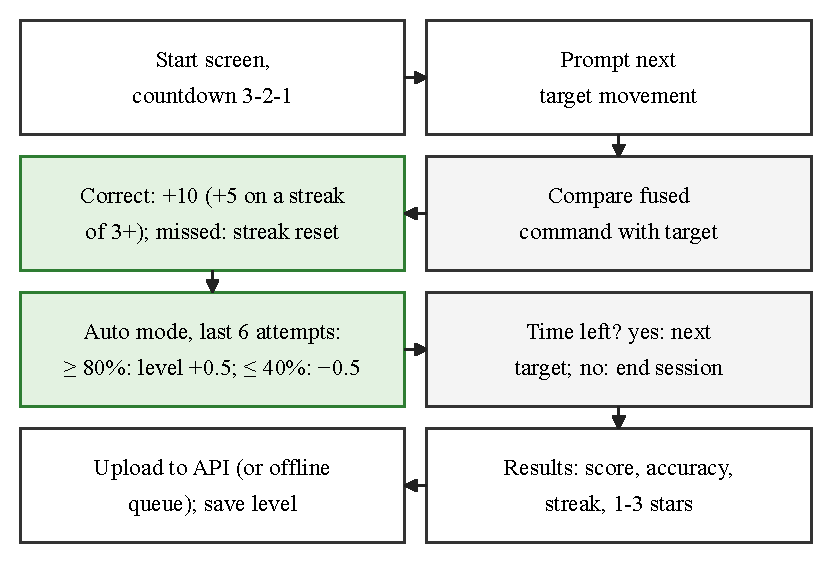
\includegraphics[width=0.92\columnwidth]{figures/fig5_session.pdf}
\caption{Game session flow with automatic difficulty adaptation}\label{fig:session}
\end{figure}

\subsection{Web Application and Data Privacy}\label{ss:web}

The web application, RehabHub, uses React and TypeScript with the FastAPI server and SQLite database (32 endpoints). Its pages show overview statistics and patients needing attention; coded patient records with clinical notes, progress, accuracy by movement, EMG activity by movement, session history and CSV export; every session and attempt; a game launcher that selects the patient, game, input mode, difficulty and duration and shows the live log; an EMG data viewer; and settings. To protect health data, every component runs on one computer and the server listens only on the local address. Patients are identified only by coded IDs, and no camera video is stored. Login with separate roles, encryption and a security review are required before any remote or clinical use.

\subsection{Testing and Evaluation Plan}

Forty-seven automated tests cover features and filtering, fusion, the server, the offline queue, difficulty, dataset loading, EMG replay and all four games played with scripted input on a hidden display. Recorded EMG can be replayed into the live pipeline, so the full system can be tested without the sensor. The planned evaluation has three stages: five to ten healthy volunteers for webcam detection accuracy, accuracy using \eqref{eq:ma} and camera to game delay (target median below 300~ms); a usability study with the System Usability Scale~\cite{brooke1996} (target above 68); and, after ethics approval, a small pilot with stroke patients.

% =====================================================================
\section{Results and Discussion}

\subsection{EMG Activity per Movement}\label{ss:res-act}

Table~\ref{tab:activity} shows the mean window RMS per movement over the nine volunteers. Hand Close produces by far the most activity and Rest the least, the four directions lie close together, and Hand Open is only about twice Rest. Relative to each volunteer's own Rest, Hand Close ranged from 7.3 times (S03) to 117 times (S02), showing large differences in gain and electrode contact between people.

\begin{table}[!t]
\caption{Mean EMG activity per movement (9 volunteers)}\label{tab:activity}
\tablefont
\begin{tabularx}{\columnwidth}{|Y|C{26mm}|C{18mm}|}
\hline
\hd{Movement} & \hd{Mean RMS (ADC units)} & \hd{Ratio to Rest}\\\hline
Hand Close & 884.6 & 23.0\\\hline
Up / Down & 413.8 / 413.5 & 10.7 / 10.7\\\hline
Right / Left & 387.9 / 301.4 & 10.1 / 7.8\\\hline
Hand Open & 92.0 & 2.4\\\hline
Rest & 38.5 & 1.0\\\hline
\end{tabularx}
\end{table}

\subsection{Classification Performance}\label{ss:res-class}

Table~\ref{tab:results} compares all methods on the same splits. With 200~ms windows the best classical model, the SVM, reached 37.2\% LOSO accuracy, well above chance but far from usable for game control. The same features on 5.12~s windows raised the SVM to 47.3\%. The untouched MOMENT-1 model was at chance, but its frozen embeddings with a random forest gave the best LOSO result, 48.1\% (macro F1 0.443). Fine-tuning did not beat frozen features: the linear probe reached 43.0\% and LoRA 43.2\%. Replacing the per-subject calibration with RevIN lowered the frozen models by 11--13 points.

\begin{table}[!t]
\caption{Accuracy over 7 movements (chance 14.3\%)}\label{tab:results}
\tablefont
\begin{tabularx}{\columnwidth}{|Y|C{10mm}|C{10mm}|C{12mm}|}
\hline
\hd{Method} & \hd{LOSO} & \hd{LOSO F1} & \hd{Holdout}\\\hline
LDA, 200 ms & 34.7\% & 0.297 & 36.0\%\\\hline
SVM, 200 ms & 37.2\% & 0.321 & 40.5\%\\\hline
Random forest, 200 ms & 34.0\% & 0.307 & 37.5\%\\\hline
LDA, 5.12 s & 43.8\% & 0.381 & 40.3\%\\\hline
SVM, 5.12 s & 47.3\% & 0.425 & \textbf{50.2\%}\\\hline
Random forest, 5.12 s & 40.3\% & 0.368 & 45.0\%\\\hline
MOMENT, untrained head & 14.2\% & 0.059 & 17.4\%\\\hline
Frozen MOMENT + LDA & 41.9\% & 0.392 & 45.2\%\\\hline
Frozen MOMENT + SVM & 46.4\% & 0.425 & 48.3\%\\\hline
Frozen MOMENT + RF & \textbf{48.1\%} & \textbf{0.443} & 49.3\%\\\hline
Frozen MOMENT + RF, RevIN & 35.3\% & 0.304 & 29.2\%\\\hline
MOMENT linear probe & 43.0\% & 0.369 & 45.5\%\\\hline
MOMENT LoRA & 43.2\% & 0.369 & 45.5\%\\\hline
\end{tabularx}
\end{table}

\subsection{Per-Movement Results and Public Data}

Every method recognized Rest, Hand Open and Hand Close far better than the directions (Table~\ref{tab:recall}). Longer windows and MOMENT features mainly improved Hand Open (46\% to 74\%) and Hand Close, while Up and Down stayed near chance. Accuracy also varied strongly between volunteers: S03 was hardest for every method (16--31\%), and S05 and S06 easiest (up to 58.5\%), so differences of one or two points between the best methods are within this spread. The public UCI data did not raise the best accuracy. As extra windows it lowered the SVM by 4.2 and LoRA by 4.1 points, because it covers only three of our movements; pre-training LoRA on it gave +1.2 points on average (44.4\%), mostly from one volunteer. Its armband sensor and short gestures differ too much from our recordings to replace data from our own sensor.

\begin{table}[!t]
\caption{LOSO recall per movement (Frozen + RF: frozen MOMENT-1 features with a random forest)}\label{tab:recall}
\tablefont
\begin{tabularx}{\columnwidth}{|Y|C{10mm}|C{10mm}|C{13mm}|C{9mm}|}
\hline
\hd{Movement} & \hd{SVM 200 ms} & \hd{SVM 5.12 s} & \hd{Frozen + RF} & \hd{LoRA}\\\hline
Rest & 81\% & 74\% & 78\% & 72\%\\\hline
Hand Open & 46\% & 59\% & 74\% & 74\%\\\hline
Hand Close & 66\% & 79\% & 75\% & 76\%\\\hline
Left & 23\% & 47\% & 40\% & 32\%\\\hline
Right & 9\% & 40\% & 31\% & 18\%\\\hline
Up & 19\% & 23\% & 9\% & 19\%\\\hline
Down & 11\% & 5\% & 27\% & 3\%\\\hline
\end{tabularx}
\end{table}

\subsection{Implemented System}

The parts were checked by the authors to work together: the battery powered sensor and ESP32 stream timestamped samples over USB; the webcam module detects the seven movements and the pointer in real time; the fusion engine attaches EMG features to every command; the four games run with rewards and automatic difficulty; sessions are stored or queued and uploaded later; and the physiotherapist can launch games and review patients, sessions and EMG activity. All 47 tests pass. These were functional checks only. Each command carries its frame capture time and the games log the camera to game delay, but this delay, webcam detection accuracy and usability have not yet been measured. By design, a command is produced every 50~ms and a new EMG window every 100~ms.

\subsection{Discussion}

Using one EMG channel for activity and a webcam for hand position keeps the hardware low cost (about LKR 14,000), easy to wear and free of inertial sensor calibration, which matters for home use. The results show the trade off clearly: one envelope channel separates activity levels well but carries little direction information, so the camera decides every game movement and EMG serves as activity feedback and a record of effort. Three further findings guide future work. First, window length mattered more than the model: the same SVM gained 10.1 points from 200~ms to 5.12~s windows, which are too slow for control but suit session level measures of effort. Second, frozen MOMENT-1 features were the best overall, while LoRA, trained on about 1,900 windows from six people per fold, had too little data to improve on them. Third, keeping the activity level is essential: RevIN, which removes it, cost 11--13 points, so a short calibration recording per patient is a natural next step. Multi channel systems report higher accuracy under controlled conditions~\cite{jiang2018}, but our results come from one low cost channel at 100~Hz with strict testing on new people, so a direct comparison is not fair. They agree with how comparable systems use EMG, to reward or monitor muscle activity rather than to recognize several gestures~\cite{marin2021,ibrahim2024}.

\subsection{Limitations}

The classifiers were trained and tested on nine healthy volunteers, two with a missing movement, and may not generalize to other users or to stroke patients; no stroke patient data are used in this paper. The dataset was recorded at 100~Hz while the live firmware samples at 1~kHz, so offline models need resampling before live use. The webcam rules were tuned by hand and their accuracy, the latency and the usability are not yet measured. The prototype runs on one computer without login or messaging, so remote monitoring is not yet possible, and the data link is still a USB cable.

% =====================================================================
\section{Conclusion}

This paper presented a low cost, gamified upper limb stroke rehabilitation system that combines webcam hand tracking with a single channel EMG sensor, four rehabilitation games with adaptive difficulty, and a physiotherapist web application. The hardware, movement detection, fusion, games, data storage and web application work together, and an offline comparison showed that frozen MOMENT-1 features with a random forest reach 48.1\% LOSO accuracy over seven movements, with rest and hand opening and closing recognized far better than wrist directions. A single EMG channel is therefore best used for activity feedback while the camera recognizes the movement. The results do not yet show clinical benefit. Future work will add patient login and patient--physiotherapist messaging, Wi-Fi transmission and an enclosure, record more volunteers with a per-patient calibration and test a second EMG channel for directions, use EMG activity levels in the games, and carry out the three stage evaluation, including a pilot with stroke patients after ethics approval.

% =====================================================================
\section{Acknowledgements}

The authors thank the volunteers who took part in data collection. All participants were healthy adults who took part voluntarily and gave informed consent; formal ethics committee approval has not yet been obtained, and data collection from stroke patients will start only after approval. The system is a research prototype, not a certified medical device. The authors declare no conflict of interest. AI-assisted tools were used for language editing and formatting, and to help prepare the manuscript text from the authors' project documentation. The system design, implementation, data collection, experiments and analyses were carried out by the authors, who reviewed the final text and take full responsibility for it.

% =====================================================================
\stepcounter{section}
\renewcommand{\refname}{\Roman{section}.\enskip References}
\begin{thebibliography}{99}
\fontsize{9}{10.5}\selectfont
\setlength{\itemsep}{9pt}\setlength{\parsep}{0pt}
\setlength{\labelsep}{6pt}

\bibitem{gbd2024} GBD 2021 Stroke Risk Factor Collaborators, ``Global, regional, and national burden of stroke and its risk factors, 1990--2021: A systematic analysis for the Global Burden of Disease Study 2021,'' \textit{Lancet Neurol.}, vol.~23, no.~10, pp.~973--1003, 2024, doi: 10.1016/S1474-4422(24)00369-7.

\bibitem{winstein2018} C. Winstein and R. Varghese, ``Been there, done that, so what's next for arm and hand rehabilitation in stroke?'' \textit{NeuroRehabilitation}, vol.~43, no.~1, pp.~3--18, 2018, doi: 10.3233/NRE-172412.

\bibitem{doumas2021} I. Doumas \textit{et al.}, ``Serious games for upper limb rehabilitation after stroke: A meta-analysis,'' \textit{J. NeuroEng. Rehabil.}, vol.~18, no.~1, Art.~no.~100, 2021, doi: 10.1186/s12984-021-00889-1.

\bibitem{munoz2022} M. Munoz-Novoa \textit{et al.}, ``Upper limb stroke rehabilitation using surface electromyography: A systematic review and meta-analysis,'' \textit{Front. Hum. Neurosci.}, vol.~16, Art.~no.~897870, 2022, doi: 10.3389/fnhum.2022.897870.

\bibitem{zhang2020} F. Zhang \textit{et al.}, ``MediaPipe Hands: On-device real-time hand tracking,'' 2020, arXiv:2006.10214.

\bibitem{lee2018} S. I. Lee \textit{et al.}, ``Enabling stroke rehabilitation in home and community settings: A wearable sensor-based approach for upper-limb motor training,'' \textit{IEEE J. Transl. Eng. Health Med.}, vol.~6, pp.~1--11, 2018, doi: 10.1109/JTEHM.2018.2829208.

\bibitem{zondervan2016} D. K. Zondervan \textit{et al.}, ``Home-based hand rehabilitation after chronic stroke: Randomized, controlled single-blind trial comparing the MusicGlove with a conventional exercise program,'' \textit{J. Rehabil. Res. Dev.}, vol.~53, no.~4, pp.~457--472, 2016.

\bibitem{song2019} X. Song \textit{et al.}, ``Cellphone augmented reality game-based rehabilitation for improving motor function and mental state after stroke,'' in \textit{Proc. IEEE 16th Int. Conf. Wearable Implant. Body Sensor Netw. (BSN)}, 2019, pp.~1--4, doi: 10.1109/BSN.2019.8771093.

\bibitem{marin2021} O. Marin-Pardo \textit{et al.}, ``Development of a low-cost, modular muscle--computer interface for at-home telerehabilitation for chronic stroke,'' \textit{Sensors}, vol.~21, no.~5, Art.~no.~1806, 2021, doi: 10.3390/s21051806.

\bibitem{yin2018} Z.-X. Yin and H.-M. Xu, ``A wearable rehabilitation game controller using IMU sensor,'' in \textit{Proc. IEEE Int. Conf. Appl. Syst. Invention (ICASI)}, 2018, pp.~1060--1062, doi: 10.1109/ICASI.2018.8394459.

\bibitem{jiang2018} S. Jiang \textit{et al.}, ``Feasibility of wrist-worn, real-time hand, and surface gesture recognition via sEMG and IMU sensing,'' \textit{IEEE Trans. Ind. Informat.}, vol.~14, no.~8, pp.~3376--3385, 2018, doi: 10.1109/TII.2017.2779814.

\bibitem{marin2022} O. Marin-Pardo \textit{et al.}, ``Functional and neuromuscular changes induced via a low-cost, muscle--computer interface for telerehabilitation: A feasibility study in chronic stroke,'' \textit{Front. Neuroergon.}, vol.~3, Art.~no.~1046695, 2022, doi: 10.3389/fnrgo.2022.1046695.

\bibitem{lin2024} H.-P. Lin \textit{et al.}, ``A usability study on mobile EMG-guided wrist extension training in subacute stroke patients---MyoGuide,'' \textit{J. NeuroEng. Rehabil.}, vol.~21, no.~1, Art.~no.~39, 2024, doi: 10.1186/s12984-024-01334-9.

\bibitem{heins2017} S. Heins \textit{et al.}, ``Robotic-assisted serious game for motor and cognitive post-stroke rehabilitation,'' in \textit{Proc. IEEE 5th Int. Conf. Serious Games Appl. Health (SeGAH)}, 2017, pp.~1--8.

\bibitem{song2022} X. Song \textit{et al.}, ``Activities of daily living-based rehabilitation system for arm and hand motor function retraining after stroke,'' \textit{IEEE Trans. Neural Syst. Rehabil. Eng.}, vol.~30, pp.~621--631, 2022, doi: 10.1109/TNSRE.2022.3156387.

\bibitem{ibrahim2024} Z. Ibrahim \textit{et al.}, ``Enhancing upper limb stroke rehabilitation with electromyography-monitored virtual reality-based games,'' \textit{J. Robot.}, vol.~2024, Art.~no.~8945325, 2024, doi: 10.1155/2024/8945325.

\bibitem{dhuzuki2025} N. H. Mohd Dhuzuki \textit{et al.}, ``Design and implementation of a deep learning-based hand gesture recognition system for rehabilitation Internet-of-Things (RIoT) environments using MediaPipe,'' \textit{IIUM Eng. J.}, vol.~26, no.~1, pp.~353--372, 2025.

\bibitem{geng2017} Y. Geng \textit{et al.}, ``Improving the robustness of real-time myoelectric pattern recognition against arm position changes in transradial amputees,'' \textit{BioMed Res. Int.}, vol.~2017, pp.~1--10, 2017, doi: 10.1155/2017/5090454.

\bibitem{breiman2001} L. Breiman, ``Random forests,'' \textit{Mach. Learn.}, vol.~45, no.~1, pp.~5--32, 2001, doi: 10.1023/A:1010933404324.

\bibitem{panwar2019} M. Panwar \textit{et al.}, ``Rehab-Net: Deep learning framework for arm movement classification using wearable sensors for stroke rehabilitation,'' \textit{IEEE Trans. Biomed. Eng.}, vol.~66, no.~11, pp.~3026--3037, 2019, doi: 10.1109/TBME.2019.2899927.

\bibitem{goswami2024} M. Goswami \textit{et al.}, ``MOMENT: A family of open time-series foundation models,'' in \textit{Proc. 41st Int. Conf. Mach. Learn. (ICML)}, 2024, pp.~16115--16152.

\bibitem{hu2022} E. J. Hu \textit{et al.}, ``LoRA: Low-rank adaptation of large language models,'' in \textit{Proc. Int. Conf. Learn. Represent. (ICLR)}, 2022.

\bibitem{kim2022} T. Kim \textit{et al.}, ``Reversible instance normalization for accurate time-series forecasting against distribution shift,'' in \textit{Proc. Int. Conf. Learn. Represent. (ICLR)}, 2022.

\bibitem{lobov2018} S. Lobov \textit{et al.}, ``Latent factors limiting the performance of sEMG-interfaces,'' \textit{Sensors}, vol.~18, no.~4, Art.~no.~1122, 2018, doi: 10.3390/s18041122.

\bibitem{brooke1996} J. Brooke, ``SUS: A `quick and dirty' usability scale,'' in \textit{Usability Evaluation in Industry}, P. W. Jordan, B. Thomas, B. A. Weerdmeester, and I. L. McClelland, Eds. London, U.K.: Taylor \& Francis, 1996, pp.~189--194.

\end{thebibliography}

\end{document}
